\documentclass[11pt,a4paper]{article}
\usepackage[utf8]{inputenc}
\usepackage[T1]{fontenc}
\usepackage[brazilian]{babel}
\usepackage[margin=2.3cm]{geometry}
\usepackage{graphicx}
\usepackage{booktabs}
\usepackage{array}
\usepackage{xcolor}
\usepackage{hyperref}
\usepackage{caption}
\usepackage{subcaption}
\usepackage{amsmath}
\usepackage{longtable}
\usepackage{float}
\usepackage{enumitem}
\usepackage{multirow}
\usepackage{seqsplit}

\hypersetup{
  colorlinks=true,
  linkcolor=blue!50!black,
  urlcolor=blue!50!black,
  citecolor=blue!50!black
}

\title{Predição de Trip de Óleo Lubrificante na Turbina A\\
\large Metodologia, modelo vencedor (EXP16) e por que 2 dos 3 casos\\
conhecidos não têm sinal antecipado disponível}
\author{Pipeline \texttt{cnn1d\_ae} (AutoML) --- projeto \texttt{TesteMLCab} (Cabiunas/Petrobras)}
\date{Agosto de 2026}

\begin{document}
\maketitle

\begin{abstract}
Este relatório documenta o EXP16: uma nova frente de detecção de anomalias,
independente da linha de trabalho da temperatura T5, focada em prever o
alarme de trip por baixa pressão de óleo lubrificante do compressor
(\texttt{PALL\_6240309}, sensor \texttt{954005\_624\_PI\_0308}). Um grid
amplo de AutoML (840 combinações de modelo/threshold/debounce, EXP16a)
selecionou o \textbf{IsolationForest} como modelo vencedor, operando sobre
um grupo multivariado simples (o próprio sensor-alvo mais os 10 canais de
vibração da turbina). O candidato final (EXP16b) atinge \textbf{hit\_rate
de 100\% (2/2) no período de teste} com falso alerta de apenas
\textbf{0,143\%} e variância de semente nula. Uma investigação mais
cuidadosa da \emph{antecedência real} de cada detecção, no entanto, revelou
que apenas \textbf{1 dos 3 eventos genuínos conhecidos} do histórico
(2024-03-07, 2025-11-04, 2026-02-26) tem de fato um precursor mensurável --
o episódio de 2025-11-04, detectado com \textbf{$\sim$14,3 horas de
antecedência}. Os outros dois eventos foram investigados a fundo, inclusive
com duas hipóteses concretas de sinal precursor levantadas e testadas
(declínio de temperatura do óleo/mancais e elevação da pressão diferencial
de vazamento de gás de selagem, \texttt{PDIT\_0305}) -- \textbf{ambas
refutadas} com evidência quantitativa. A conclusão é que, com a
instrumentação disponível hoje, a cobertura genuinamente preditiva desse
alarme está limitada a $\sim$1 em 3 casos, um limite de informação física
e não de modelagem.
\end{abstract}

\tableofcontents

\section{Introdução e contexto}

O projeto de detecção de anomalias da Turbina A concentrou seus primeiros
experimentos (EXP1--EXP15) no sensor de temperatura T5 (\texttt{TC382\_03\_A}),
alcançando um candidato AutoML de referência com 92,5\% de cobertura de
alarme (EXP10c) e um candidato CNN1D-Autoencoder consolidado com 77,5\%
(EXP15b). Este relatório abre uma frente nova, \textbf{independente}: em
vez de temperatura, o alvo é o circuito de óleo lubrificante do compressor,
motivado pela pergunta ``conseguimos prever também os alarmes de
\emph{trip} (desligamento por proteção), não só os de alta temperatura?''

\subsection{Por que este alvo, e não os outros dois trips de óleo}

A planilha de alarmes da Turbina A tem 3 tags com ``TRIP'' na descrição, todos
do circuito de óleo lubrificante:

\begin{center}
\begin{tabular}{lll}
\toprule
Tag do alarme & Descrição & Situação como alvo \\
\midrule
\texttt{PALL\_6240340} & Pressão baixa óleo header (proteção turbina) & descartado \\
\texttt{TALL\_6240325} & Temperatura baixa tanque óleo & descartado \\
\texttt{PALL\_6240309} & Pressão baixa óleo header compressor & \textbf{escolhido} \\
\bottomrule
\end{tabular}
\end{center}

Cruzando cada um dos $13$ eventos históricos desses 3 alarmes com o estado
operacional da turbina (\texttt{RUNNING\_A}) no instante exato do disparo,
verificou-se que \texttt{PALL\_6240340} e \texttt{TALL\_6240325} disparam em
$99$--$100\%$ dos casos com a turbina \textbf{já parada} -- ou seja, o
sensor já havia colapsado para o valor de desligamento antes do alarme
soar. São consequência do desligamento, não uma falha incipiente a prever.
Já \texttt{PALL\_6240309} tem 3 de 7 eventos (dentro do período com dado de
sensor disponível, 2024--2026) ocorrendo com a turbina genuinamente em
operação -- por isso foi o único escolhido como alvo de predição.

\section{Metodologia}

\subsection{Dados}

\begin{itemize}[leftmargin=1.4em]
  \item \textbf{Sensores}: dataset ClearML \texttt{Cabiunas full 2024-2026 30s}
  (id \texttt{a97ba56ba14840fbb1125c2a82f883c9}), granularidade de 30 segundos,
  cobrindo 2024-01-01 a 2026-04-30 ($\sim$2,45 milhões de pontos).
  \item \textbf{Alarmes}: catálogo \texttt{alarmes\_selecionados\_turbina\_a.csv},
  2022--2026, filtrado para eventos \texttt{ACT} (ativação) do tag
  \texttt{PALL\_6240309}.
  \item \textbf{Ampliar a janela para antes de 2024?} Investigado e
  descartado: existe um dataset mais amplo (\texttt{Cabiunas consolidado
  2022-2026}) mas o ano de 2023 -- que teria os 6 eventos adicionais do
  alarme -- está com \textbf{zero linhas de dado de sensor} nesse dataset.
  2022 tem ótima cobertura, mas nenhum evento do alarme ocorreu naquele
  ano. Ampliar a janela não resolveria o gargalo de eventos genuínos de
  teste.
\end{itemize}

\subsection{Grupo multivariado e correlação}

Testou-se se sensores adicionais do mesmo circuito de óleo ajudariam a
explicar o comportamento do alvo. Por correlação (em estado ``on'', $n
\approx 1{,}65$M pontos):

\begin{center}
\begin{tabular}{lc}
\toprule
Sensor & Correlação com \texttt{PI\_0308} \\
\midrule
\texttt{954005\_624\_PI\_0340} (outra pressão do header) & 0,898 \\
\texttt{954005\_624\_PI\_0339} (terceira pressão do óleo lub.) & 0,895 \\
\texttt{954005\_624\_TI\_0325} (temp. tanque óleo) & 0,531 \\
\texttt{954005\_624\_TI\_0301/0303/0305/0307} (temp. mancais) & 0,44--0,65 \\
\texttt{TV\_35X\_A} (10 canais de vibração) & 0,12--0,51 \\
\bottomrule
\end{tabular}
\end{center}

Dois grupos foram comparados de ponta a ponta: um grupo \emph{controle}
(alvo + os 10 canais de vibração) e um grupo \emph{multivariado completo}
(+ as pressões/temperaturas do óleo listadas acima). O resultado, detalhado
na Seção~\ref{sec:modelo}, mostrou que \textbf{o grupo completo não supera
o grupo simples} -- por isso o candidato final usa apenas alvo + vibração.

\subsection{Split treino/teste (OOS)}

Split temporal em \texttt{2025-07-01}: o modelo só aprende ``normal'' com
dados anteriores a essa data (excluindo também $\pm 24$h ao redor de
qualquer alarme e períodos fora do estado ``on''); a avaliação de
\texttt{hit\_rate}/falso-alerta só considera o período posterior, nunca
visto pelo modelo. Isso deixa exatamente \textbf{2 alarmes genuínos} no
conjunto de teste (2025-11-04 e 2026-02-26) -- um terceiro evento genuíno
conhecido (2024-03-07) cai no período de treino e nunca é avaliado
formalmente, mas foi investigado à parte na Seção~\ref{sec:naodetectado}.

\section{Modelo vencedor e como foi configurado}
\label{sec:modelo}

\subsection{EXP16a: grid amplo de AutoML}

Espelhando a metodologia já validada para a T5 (EXP5$\to$EXP7), rodou-se
primeiro um grid amplo em vez de partir direto para um modelo específico:

\begin{center}
\begin{tabular}{ll}
\toprule
Parâmetro & Valores testados \\
\midrule
Modelos & \texttt{dense} (autoencoder), \texttt{ocsvm}, \texttt{iforest} \\
Grade \texttt{ocsvm} & $\nu \in \{0{,}01, 0{,}03, 0{,}05, 0{,}1\}$ $\times$ $\gamma \in \{\text{scale}, \text{auto}\}$ \\
Percentis de threshold & 90; 93; 95; 97; 99; 99,5; 99,9 \\
Debounce (pontos consecutivos) & 1; 2; 3; 6; 12; 24 \\
Grupos de sensores & controle (alvo+vibração) vs. multivariado completo \\
\midrule
\textbf{Total} & \textbf{840 trials} (20 treinos reais de modelo) \\
\bottomrule
\end{tabular}
\end{center}

\begin{figure}[H]
\centering
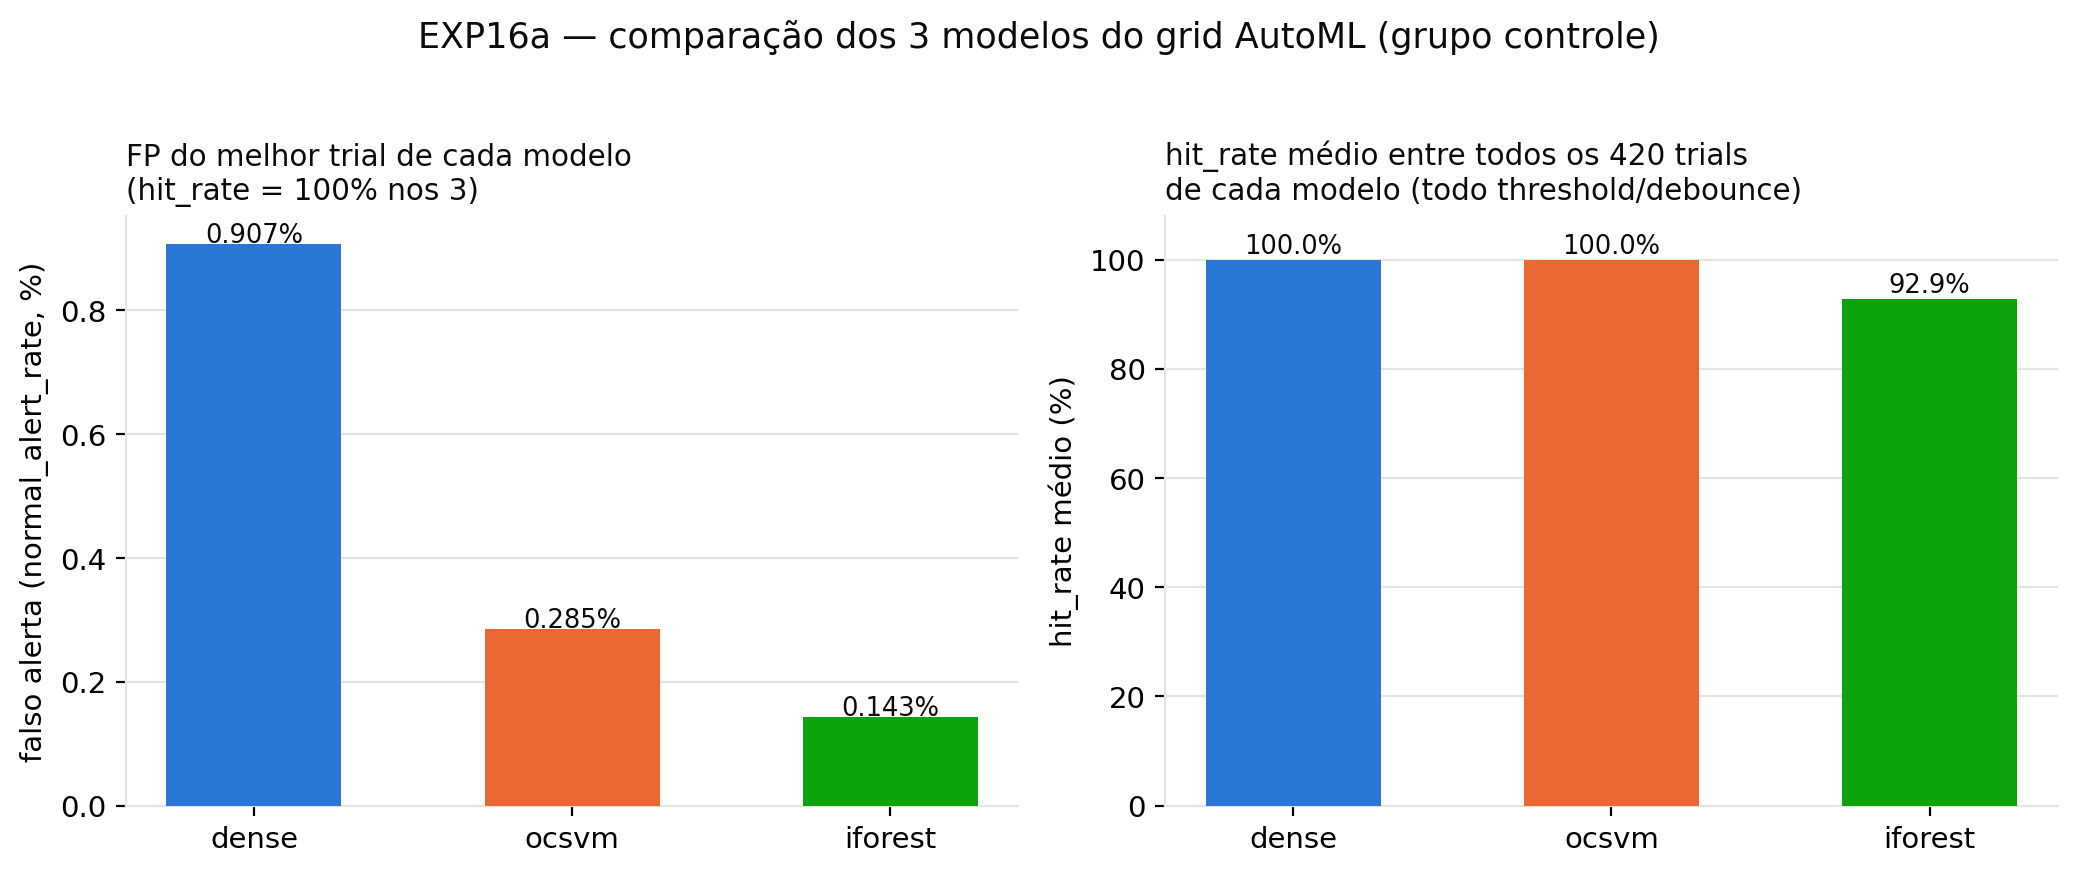
\includegraphics[width=0.92\textwidth]{fig_comparativo_modelos.png}
\caption{Comparação dos 3 modelos no grupo controle: apesar de \texttt{dense}
e \texttt{ocsvm} também atingirem hit\_rate médio de 100\% entre todos os
420 trials (contra 92,9\% do \texttt{iforest}), o \texttt{iforest} entrega
o menor falso alerta no seu melhor trial -- 0,143\%, contra 0,285\% do
\texttt{ocsvm} e 0,907\% do \texttt{dense}, mais de 6$\times$ pior.}
\label{fig:comparativo}
\end{figure}

\textbf{Vencedor: IsolationForest}, com percentil 99,5 e debounce de 24
pontos (12 minutos), no grupo \emph{controle} (alvo + vibração) -- ver
Figura~\ref{fig:comparativo}. O grupo multivariado completo produziu
resultado praticamente idêntico (FP 0,144\% vs. 0,143\%), confirmando que
as pressões/temperaturas extras do óleo não agregam poder discriminante
sobre o que a vibração já entrega.

\subsection{Configuração final do modelo (EXP16b)}

\begin{center}
\begin{tabular}{ll}
\toprule
Hiperparâmetro & Valor \\
\midrule
Modelo & \texttt{sklearn.ensemble.IsolationForest} \\
\texttt{n\_estimators} & 200 \\
\texttt{contamination} & 0,05 \\
Sensores de entrada & \texttt{PI\_0308} + 10 canais \texttt{TV\_35[1-5][X/Y]\_A} \\
Features derivadas & médias/desvios móveis em 4 escalas (6min, 1h, 4h, 24h) \\
Normalização & z-score, estatísticas calculadas só no período de treino \\
Threshold & percentil 99,5 do score de anomalia em treino \\
Regra de confirmação (debounce) & 24 pontos consecutivos acima do limiar (12 min) \\
Máscara operacional & zera anomalia fora do estado ``on'' (\texttt{RUNNING\_A}) \\
Portões de rampa/volatilidade & \textbf{nenhum} (decisão deliberada, ver abaixo) \\
Semente & \texttt{RANDOM\_SEED=42}; seed-sweep com 5 sementes (42--46) \\
\bottomrule
\end{tabular}
\end{center}

\paragraph{Por que nenhum portão de pós-processamento?}
Os experimentos de T5 usam portões de rampa e de volatilidade para suprimir
falsos alertas durante manobras de carga legítimas, já que ali a vibração é
só ruído de contexto. Aqui a lógica se inverte: o sanity-check da
Seção~\ref{sec:sanity} mostrou que é \emph{a vibração} que permite ao
\texttt{iforest} separar os eventos genuínos do ruído normal -- suprimir
anomalias durante vibração elevada arriscaria descartar exatamente o sinal
que faz o modelo funcionar. Como o falso alerta já está baixo (0,143\%,
partindo do zero, sem nenhum portão -- bem diferente do ponto de partida de
1,94\% que motivou os portões na T5), a decisão foi não adicionar essa
camada de risco sem benefício comprovado.

\begin{figure}[H]
\centering
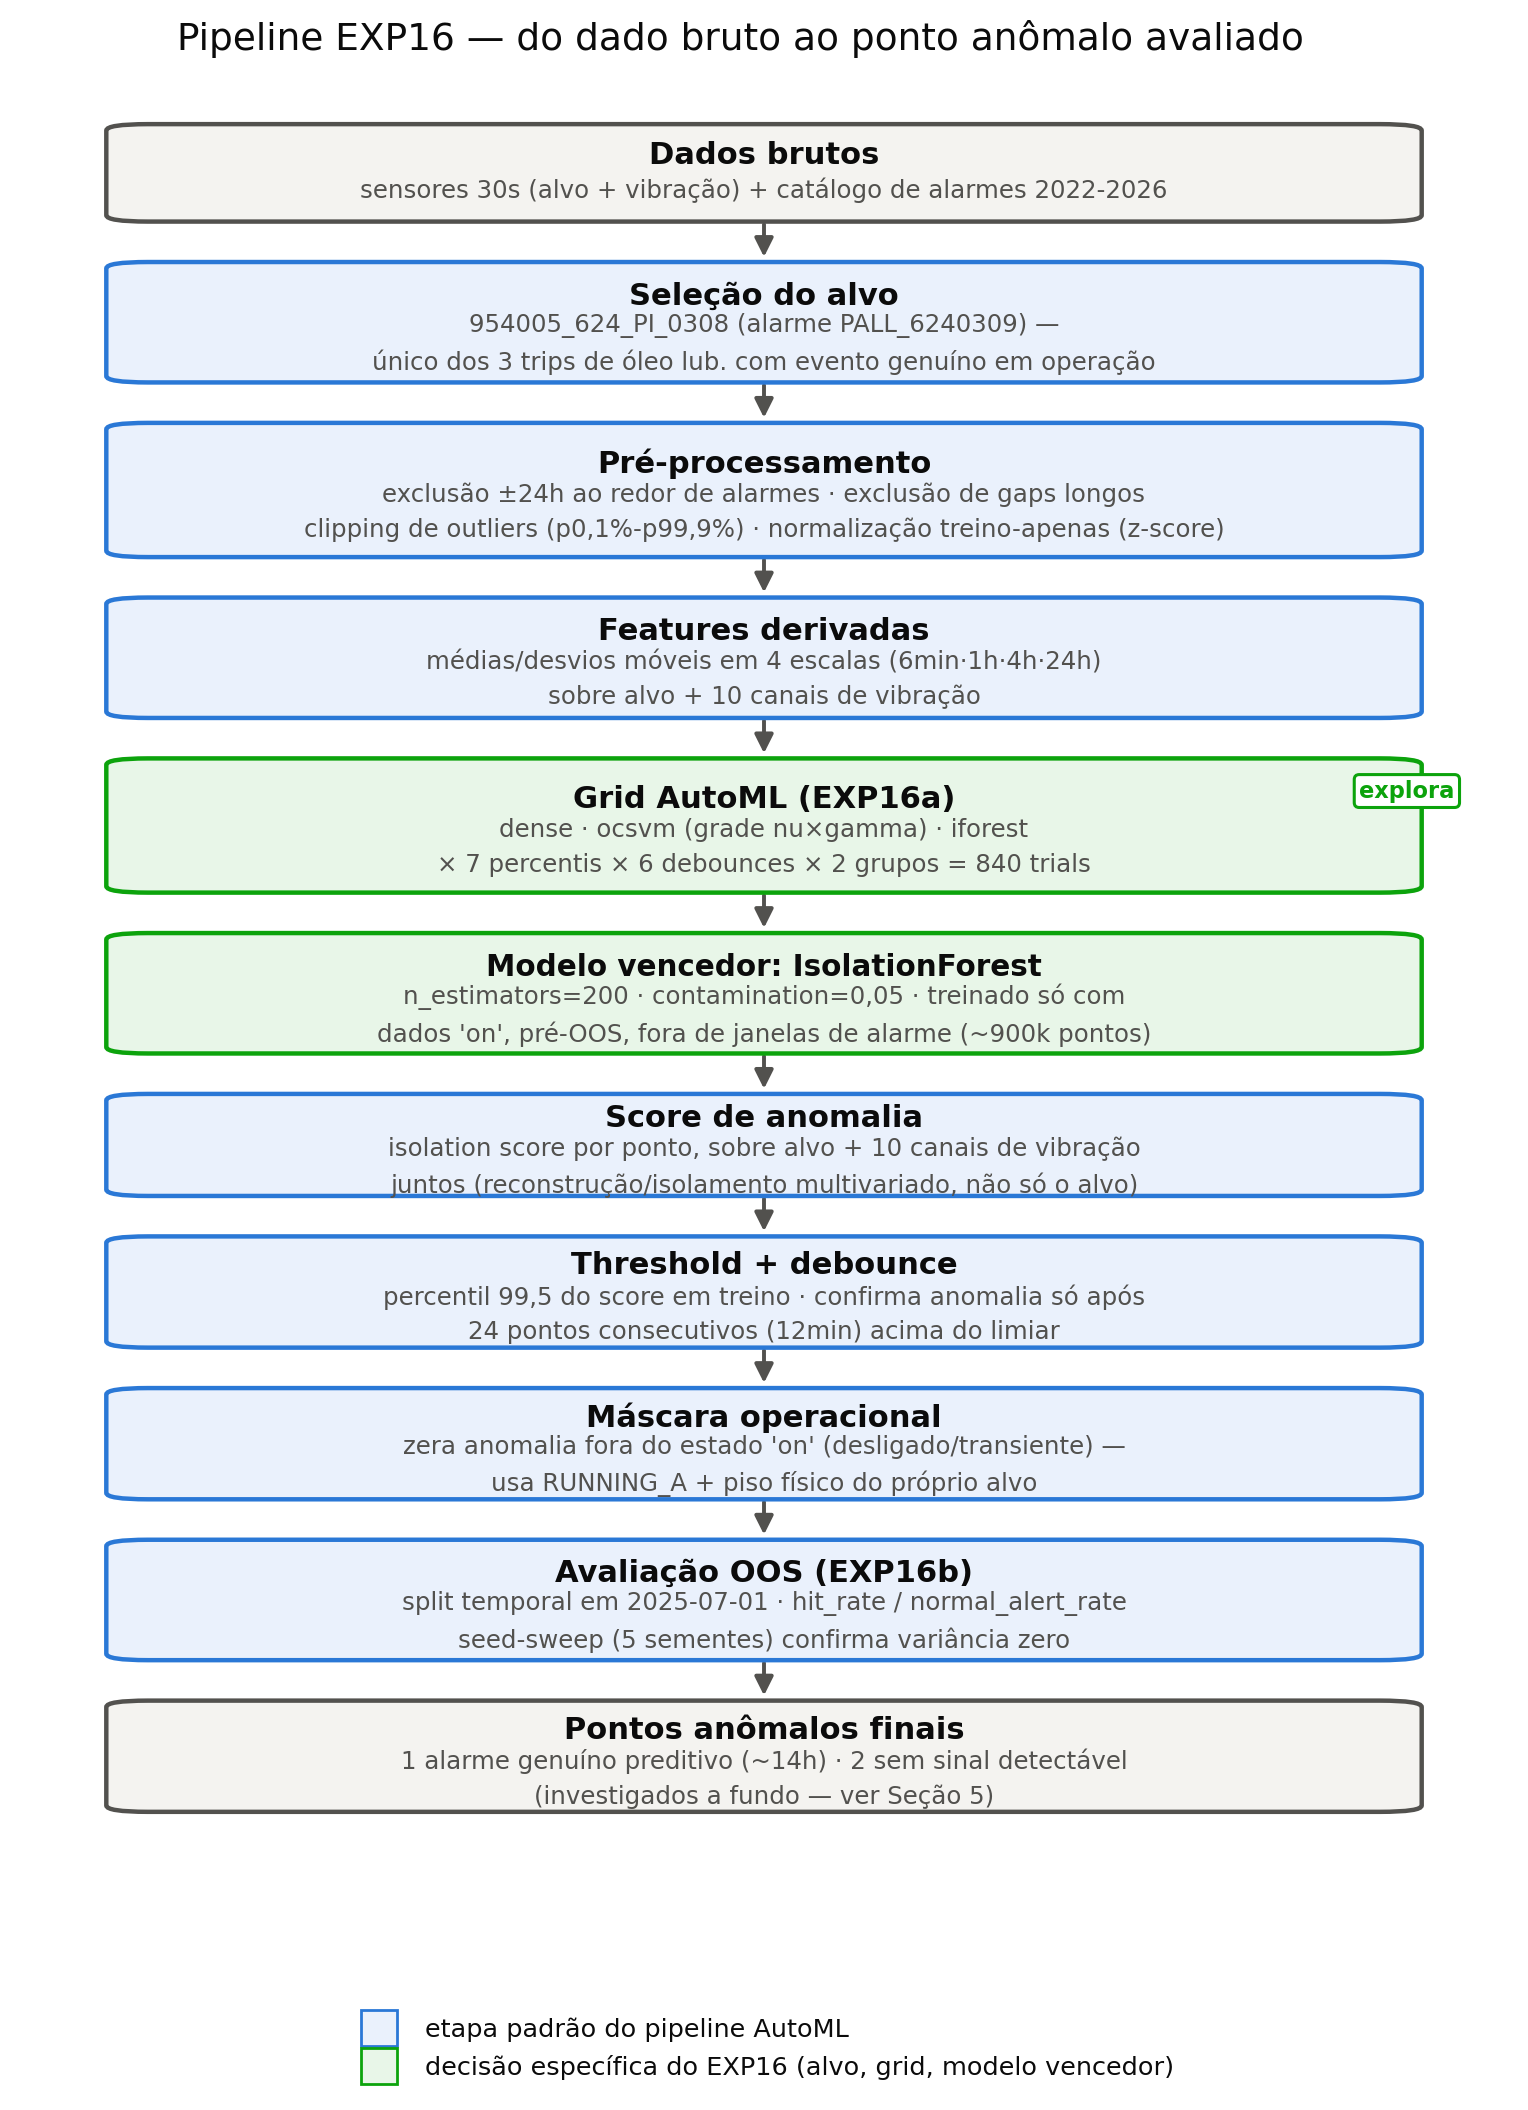
\includegraphics[width=0.85\textwidth]{fig_pipeline_exp16.png}
\caption{Esquema completo do pipeline EXP16, do dado bruto ao ponto anômalo
avaliado. Os blocos verdes marcam decisões específicas deste experimento
(escolha do alvo, grid de exploração, modelo vencedor); os azuis são etapas
padrão do framework AutoML já usado nos experimentos de T5.}
\label{fig:pipeline}
\end{figure}

\subsection{Sanity-check: o resultado é real, não artefato do conjunto pequeno}
\label{sec:sanity}

Com apenas 2 alarmes no conjunto de teste, um hit\_rate de 100\% poderia
ser um artefato -- qualquer modelo acertaria por acaso. Simulou-se então um
detector ingênuo: threshold direto sobre o valor bruto de \texttt{PI\_0308},
sem nenhum modelo, na mesma metodologia de avaliação.

\begin{center}
\begin{tabular}{lccc}
\toprule
Abordagem & Threshold & hit\_rate & Falso alerta \\
\midrule
\texttt{iforest} multivariado (vencedor) & percentil 99,5 & \textbf{100\%} & \textbf{0,143\%} \\
Ingênuo (só \texttt{PI\_0308}) & mesmo corte (p99,5) & 0\% & 1,28\% \\
Ingênuo (só \texttt{PI\_0308}) & mais frouxo (p90) & 100\% & 10,3\% (72$\times$ pior) \\
\bottomrule
\end{tabular}
\end{center}

No mesmo corte que o \texttt{iforest} usa, um threshold ingênuo erra os 2
alarmes; para acertar os 2, precisa afrouxar até um falso alerta 72$\times$
maior. Isso confirma que o \texttt{iforest} está usando o contexto conjunto
de vibração + alvo para separar os eventos com muito mais precisão do que o
valor do sensor sozinho permitiria -- o resultado é real.

\section{Resultados}

\subsection{Métricas do candidato final}

\begin{center}
\begin{tabular}{lccc}
\toprule
Métrica & Seed 42 (principal) & Média (5 sementes) & Desvio-padrão \\
\midrule
\texttt{hit\_rate} & 100\% (2/2) & \textbf{100\%} & \textbf{0,0pp} \\
Falso alerta (\texttt{normal\_alert\_rate}) & 0,143\% & 0,138\% & $\pm$0,004pp \\
\bottomrule
\end{tabular}
\end{center}

O seed-sweep (5 sementes, 42--46) confirma \textbf{variância de semente
nula} -- os 2 alarmes são detectados em todas as 5 sementes, com o falso
alerta variando só entre 0,133\% e 0,143\%. É um resultado bem mais
estável do que o CNN1D-AE jamais foi para a T5 (que tinha
\texttt{hit\_rate\_std} de vários pontos percentuais entre sementes).

\begin{figure}[H]
\centering
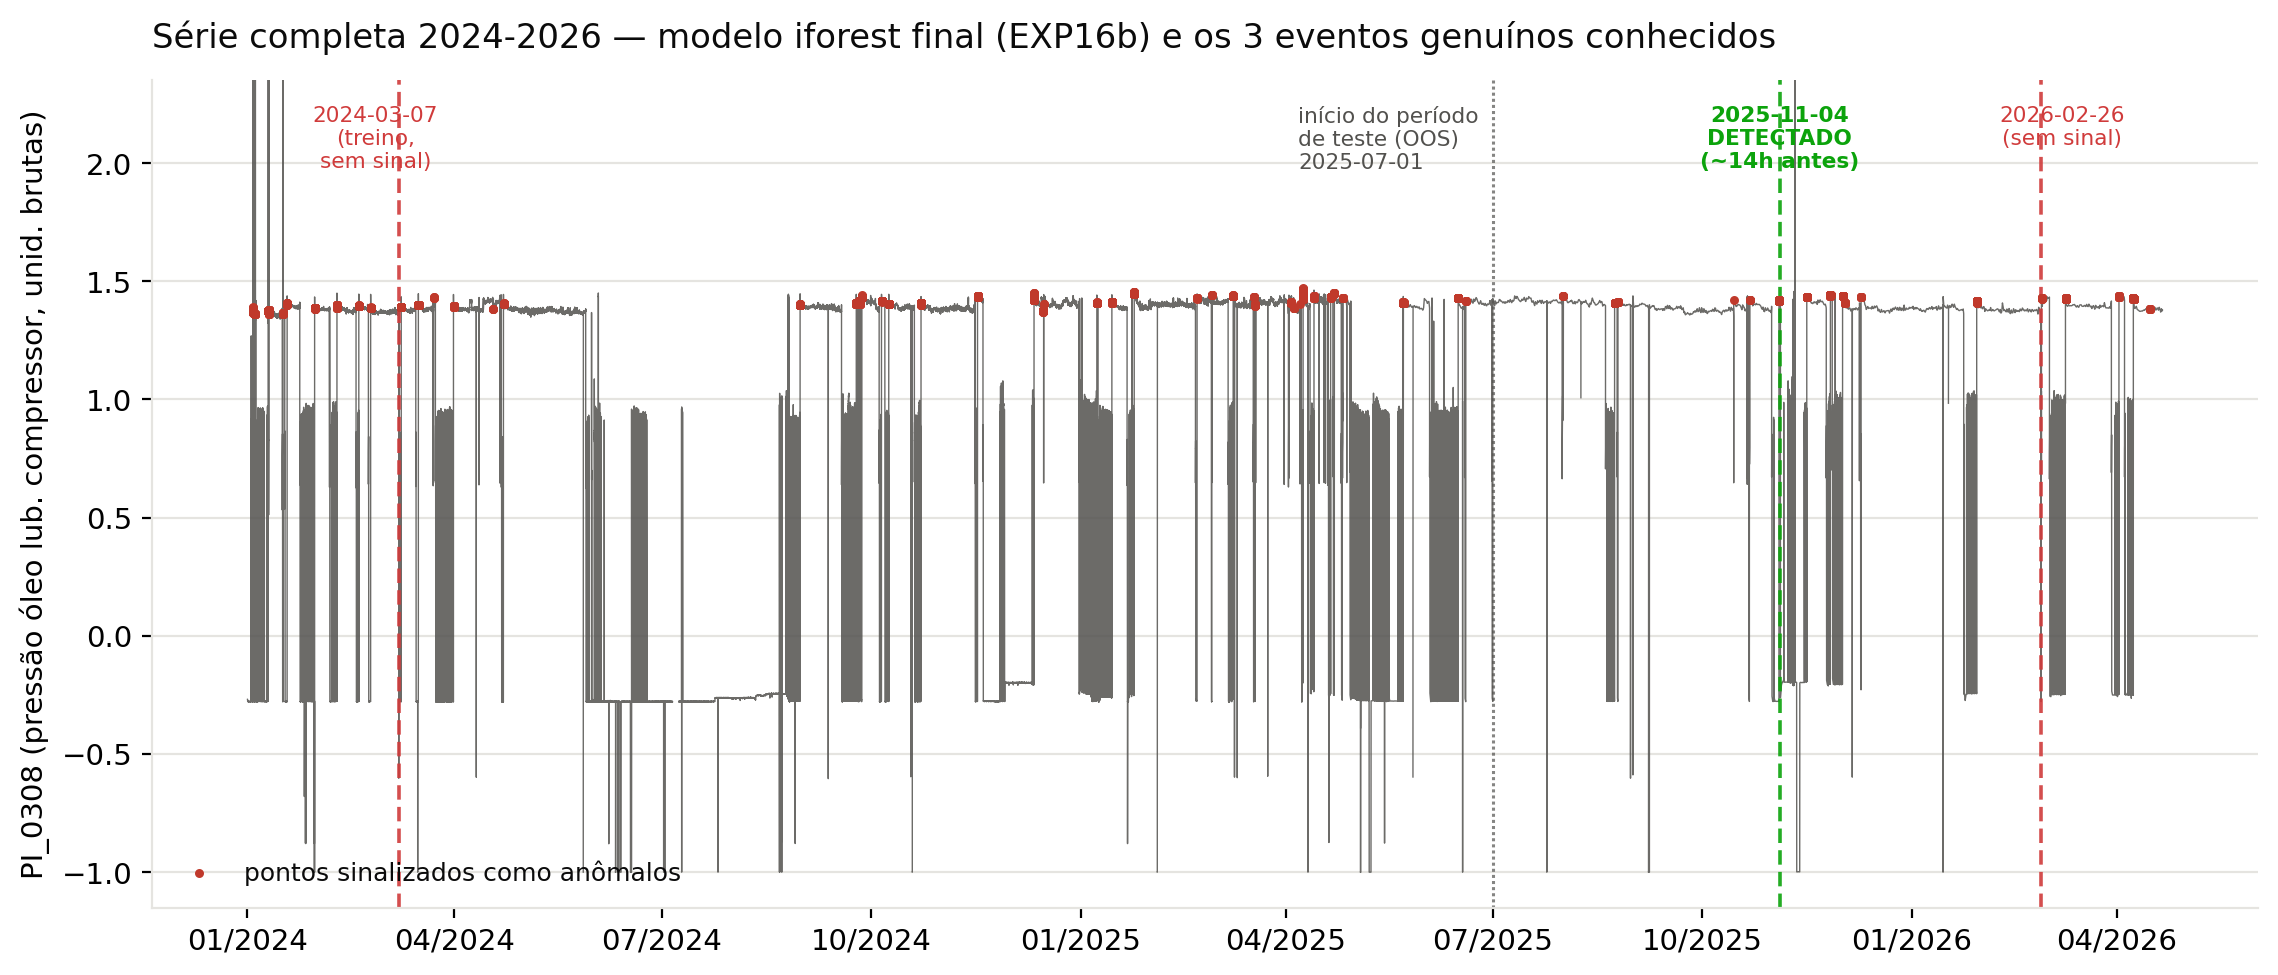
\includegraphics[width=\textwidth]{fig_serie_completa.png}
\caption{Série completa de \texttt{PI\_0308} (2024--2026) com os pontos
sinalizados como anômalos pelo modelo final (pontos vermelhos) e os 3
eventos genuínos conhecidos do alarme \texttt{PALL\_6240309} marcados. Os
grandes trechos em torno de $-0{,}25$ a $-1{,}0$ correspondem a períodos
com a turbina desligada (o sensor cai ao piso físico de leitura), excluídos
da avaliação pela máscara operacional.}
\label{fig:serie-completa}
\end{figure}

\subsection{Gráfico do acerto: o caso genuinamente preditivo}

A métrica de avaliação padrão (\texttt{eval\_alarm\_hit\_rate}) conta como
``acerto'' qualquer ponto anômalo dentro de $\pm 24$h do alarme, \textbf{antes
ou depois} -- o que pode mascarar detecção puramente reativa (útil só para
registro, não para alerta antecipado). Verificou-se então, ponto a ponto, a
antecedência \emph{real} de cada um dos 2 alarmes do conjunto de teste.

\begin{figure}[H]
\centering
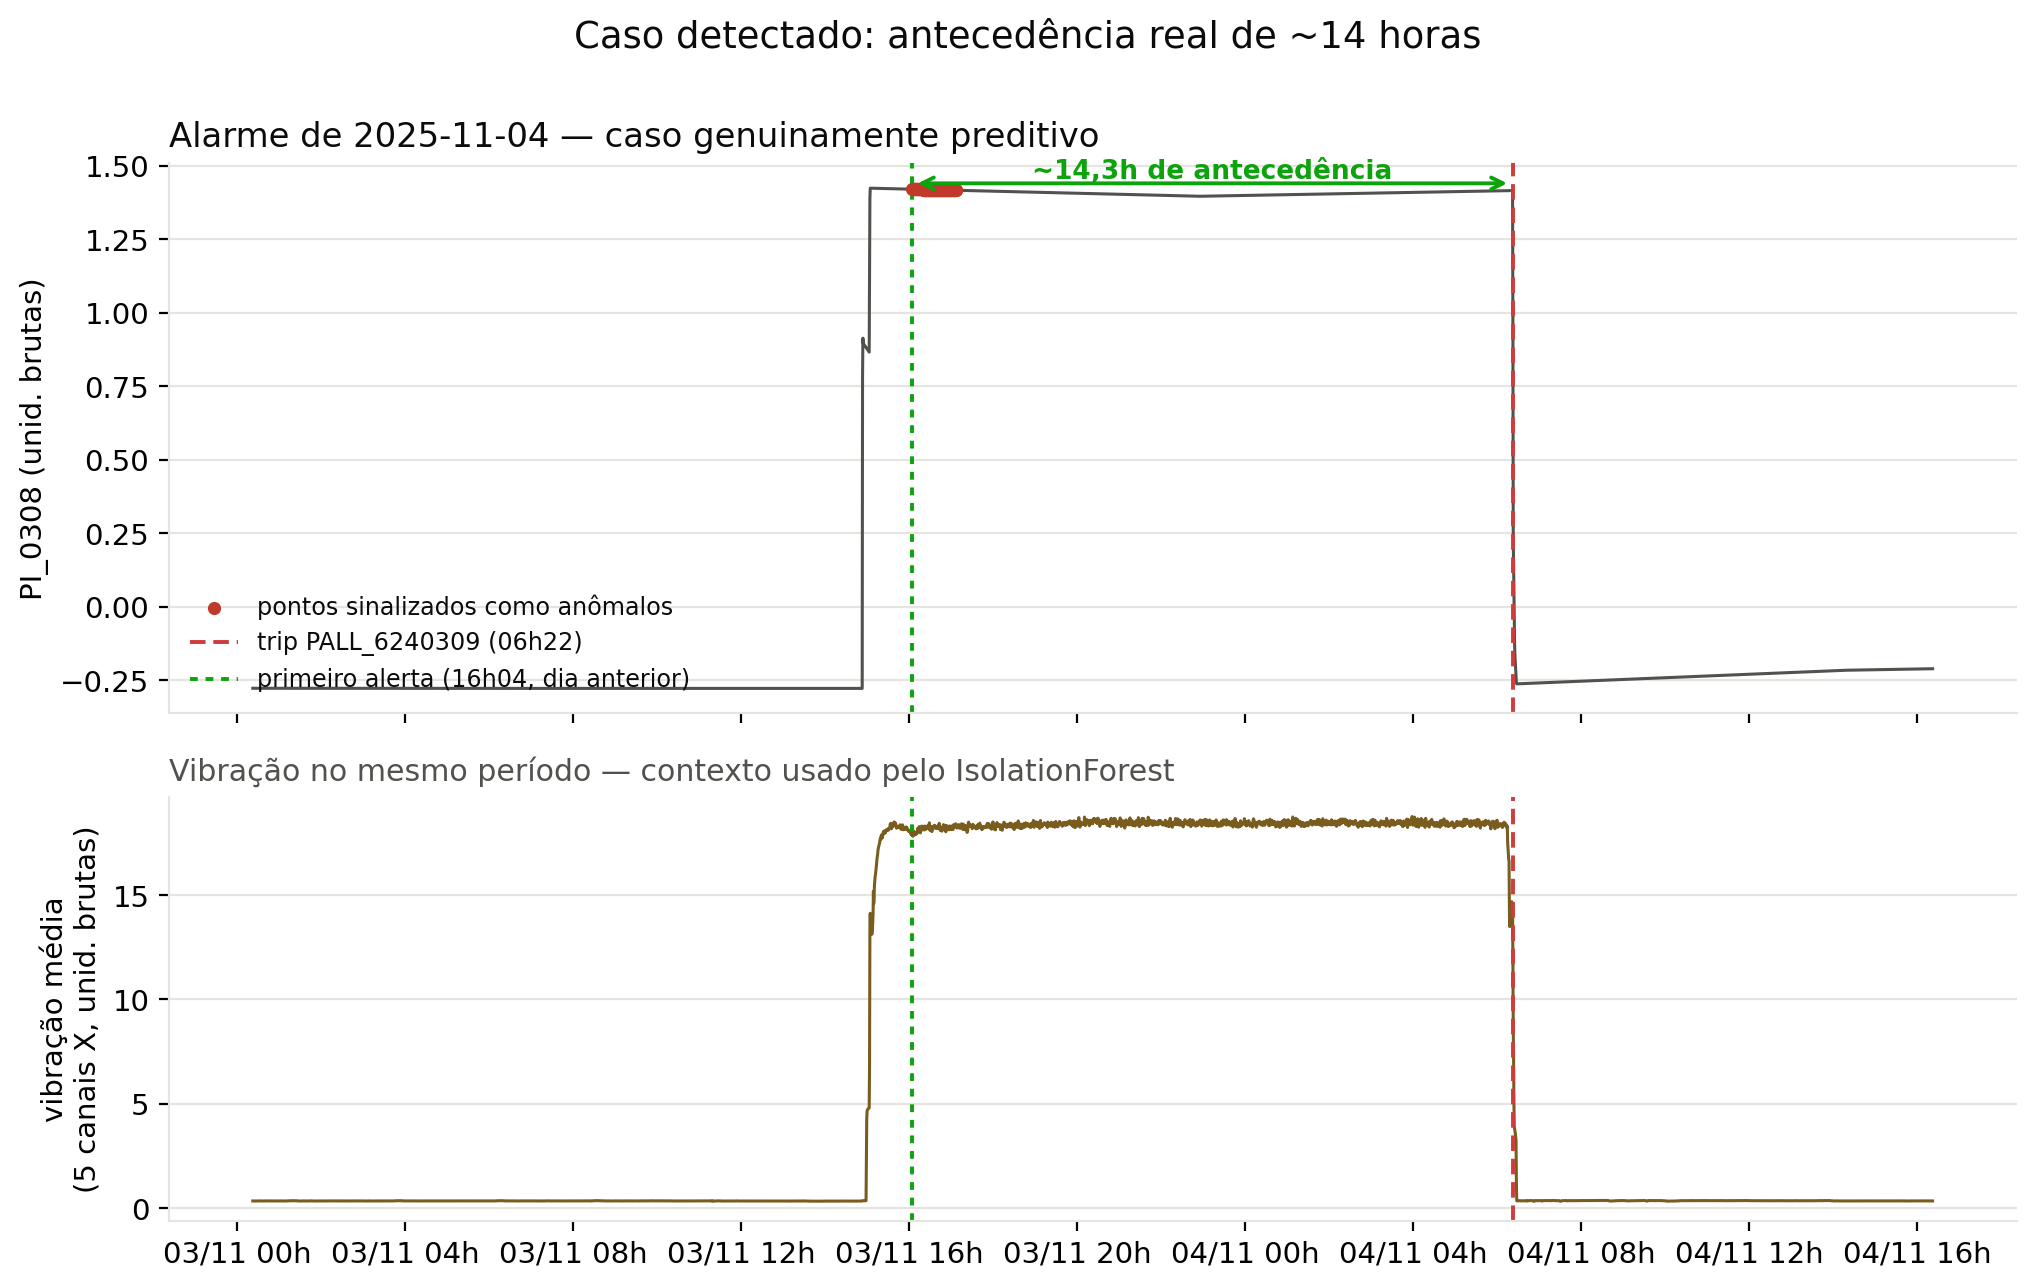
\includegraphics[width=0.92\textwidth]{fig_caso_detectado.png}
\caption{Episódio de 2025-11-04: a turbina entra em operação às $\sim$13h50
do dia anterior; o \texttt{iforest} sinaliza uma janela de anomalia
(pontos vermelhos) já entre 16h04 e 17h07 desse mesmo dia -- $\sim$14,3
horas antes do trip (linha vermelha), pouco depois da partida. É um
episódio (\emph{burst}) concentrado logo após a partida, não uma
tendência crescente ao longo de toda a janela; ainda assim, cai
inteiramente antes do trip, contando como antecedência real -- diferente
do padrão reativo descrito abaixo para os casos sem sinal.}
\label{fig:caso-detectado}
\end{figure}

\textbf{Resultado: apenas 1 dos 2 alarmes do conjunto de teste é
genuinamente preditivo.} O episódio de 2025-11-04 tem os 126 pontos
anômalos da sua janela \emph{todos antes} do trip (antecedência de 13,3 a
14,3 horas). Já o episódio de 2026-02-26 tem seus 26 pontos anômalos
\emph{todos depois} do trip (6,7 a 6,9 horas de atraso) -- um padrão
puramente reativo que, na prática, coincide com ruído de acomodação da
partida seguinte, sem valor de alerta antecipado algum.

\subsection{O que não foi previsto, e por quê}
\label{sec:naodetectado}

Checando também o terceiro evento genuíno conhecido (2024-03-07, que cai no
período de treino e nunca foi formalmente avaliado), a contagem real de
cobertura preditiva é \textbf{1 em 3 ($\sim$33\%)}, não 1 em 2:

\begin{center}
\begin{tabular}{lccc}
\toprule
Evento & Antecedência real & Classificação \\
\midrule
2024-03-07 & --- (sem sinal) & sem precursor \\
2025-11-04 & $\sim$14,3h antes & \textbf{preditivo genuíno} \\
2026-02-26 & $-6{,}7$h (depois) & sem precursor (reativo residual) \\
\bottomrule
\end{tabular}
\end{center}

\begin{figure}[H]
\centering
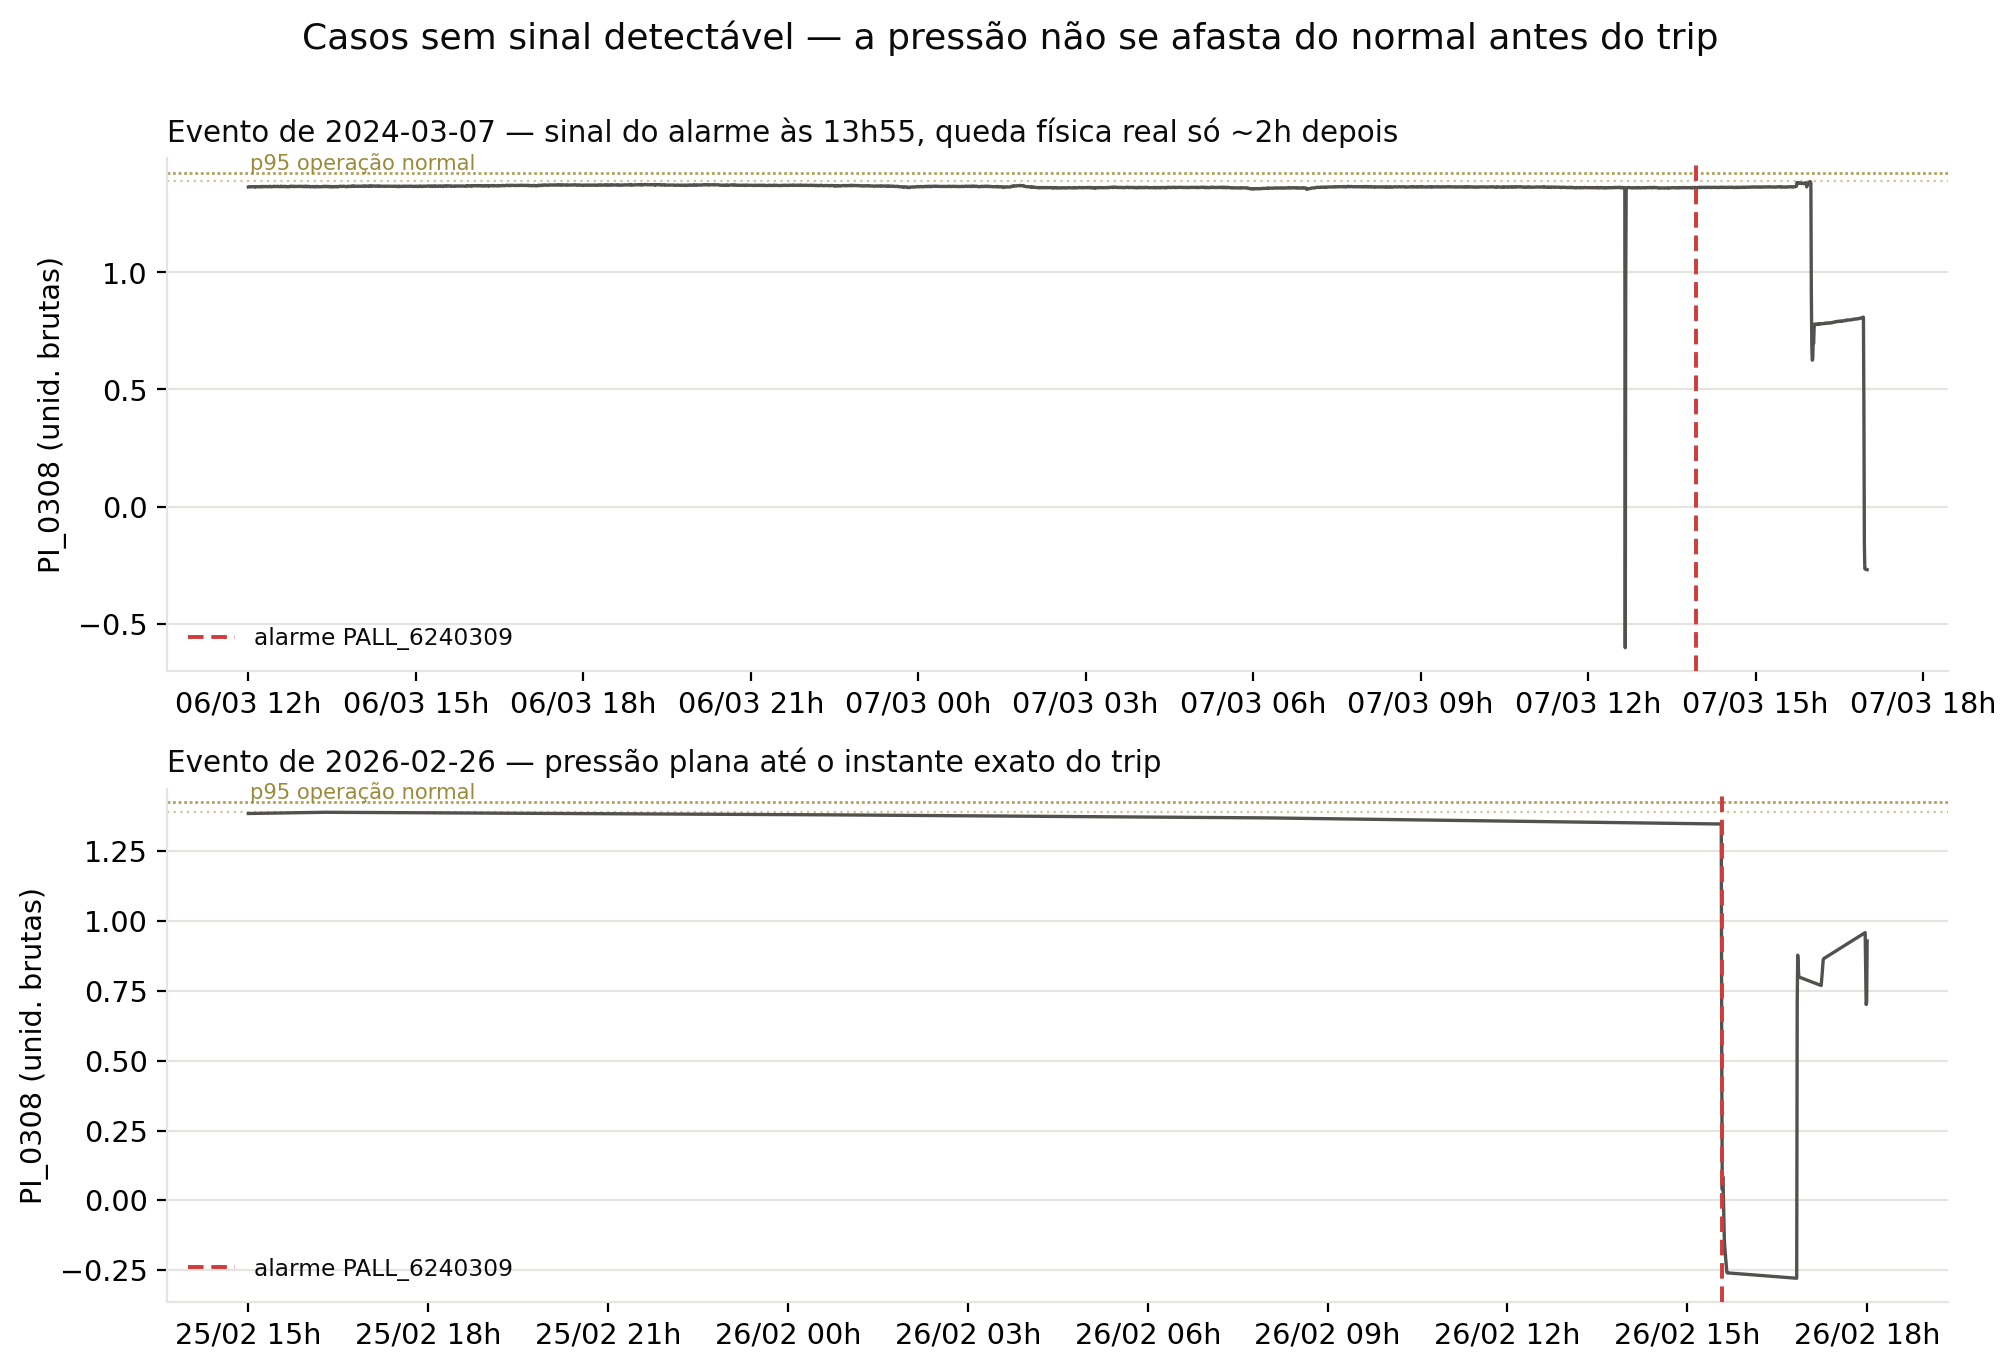
\includegraphics[width=\textwidth]{fig_casos_nao_detectados.png}
\caption{Os dois eventos sem sinal detectável. Em ambos os casos,
\texttt{PI\_0308} permanece completamente estável dentro da faixa normal
até o instante exato (ou muito próximo) do trip -- não há degradação
gradual visível em nenhum sensor disponível. No evento de 2024-03-07, o
alarme dispara às 13h55 mas a queda física real só ocorre $\sim$2h depois
(15h56), um detalhe curioso da sequência de proteção que não muda a
conclusão: não há aviso prévio detectável em nenhum dos dois casos.}
\label{fig:nao-detectados}
\end{figure}

\subsubsection{Duas hipóteses de precursor levantadas e refutadas}

Motivados a não aceitar ``sem sinal'' sem investigar, varreu-se
$\sim$36 sensores brutos disponíveis (pressões, temperaturas, deltas de
pressão) em busca de qualquer sinal diferencial nas 24h antes dos 2 casos
sem detecção, comparado contra o caso preditivo (2025-11-04) como controle.
Dois candidatos surgiram -- \textbf{e os dois foram refutados} com
evidência quantitativa, não apenas descartados por inspeção visual.

\begin{figure}[H]
\centering
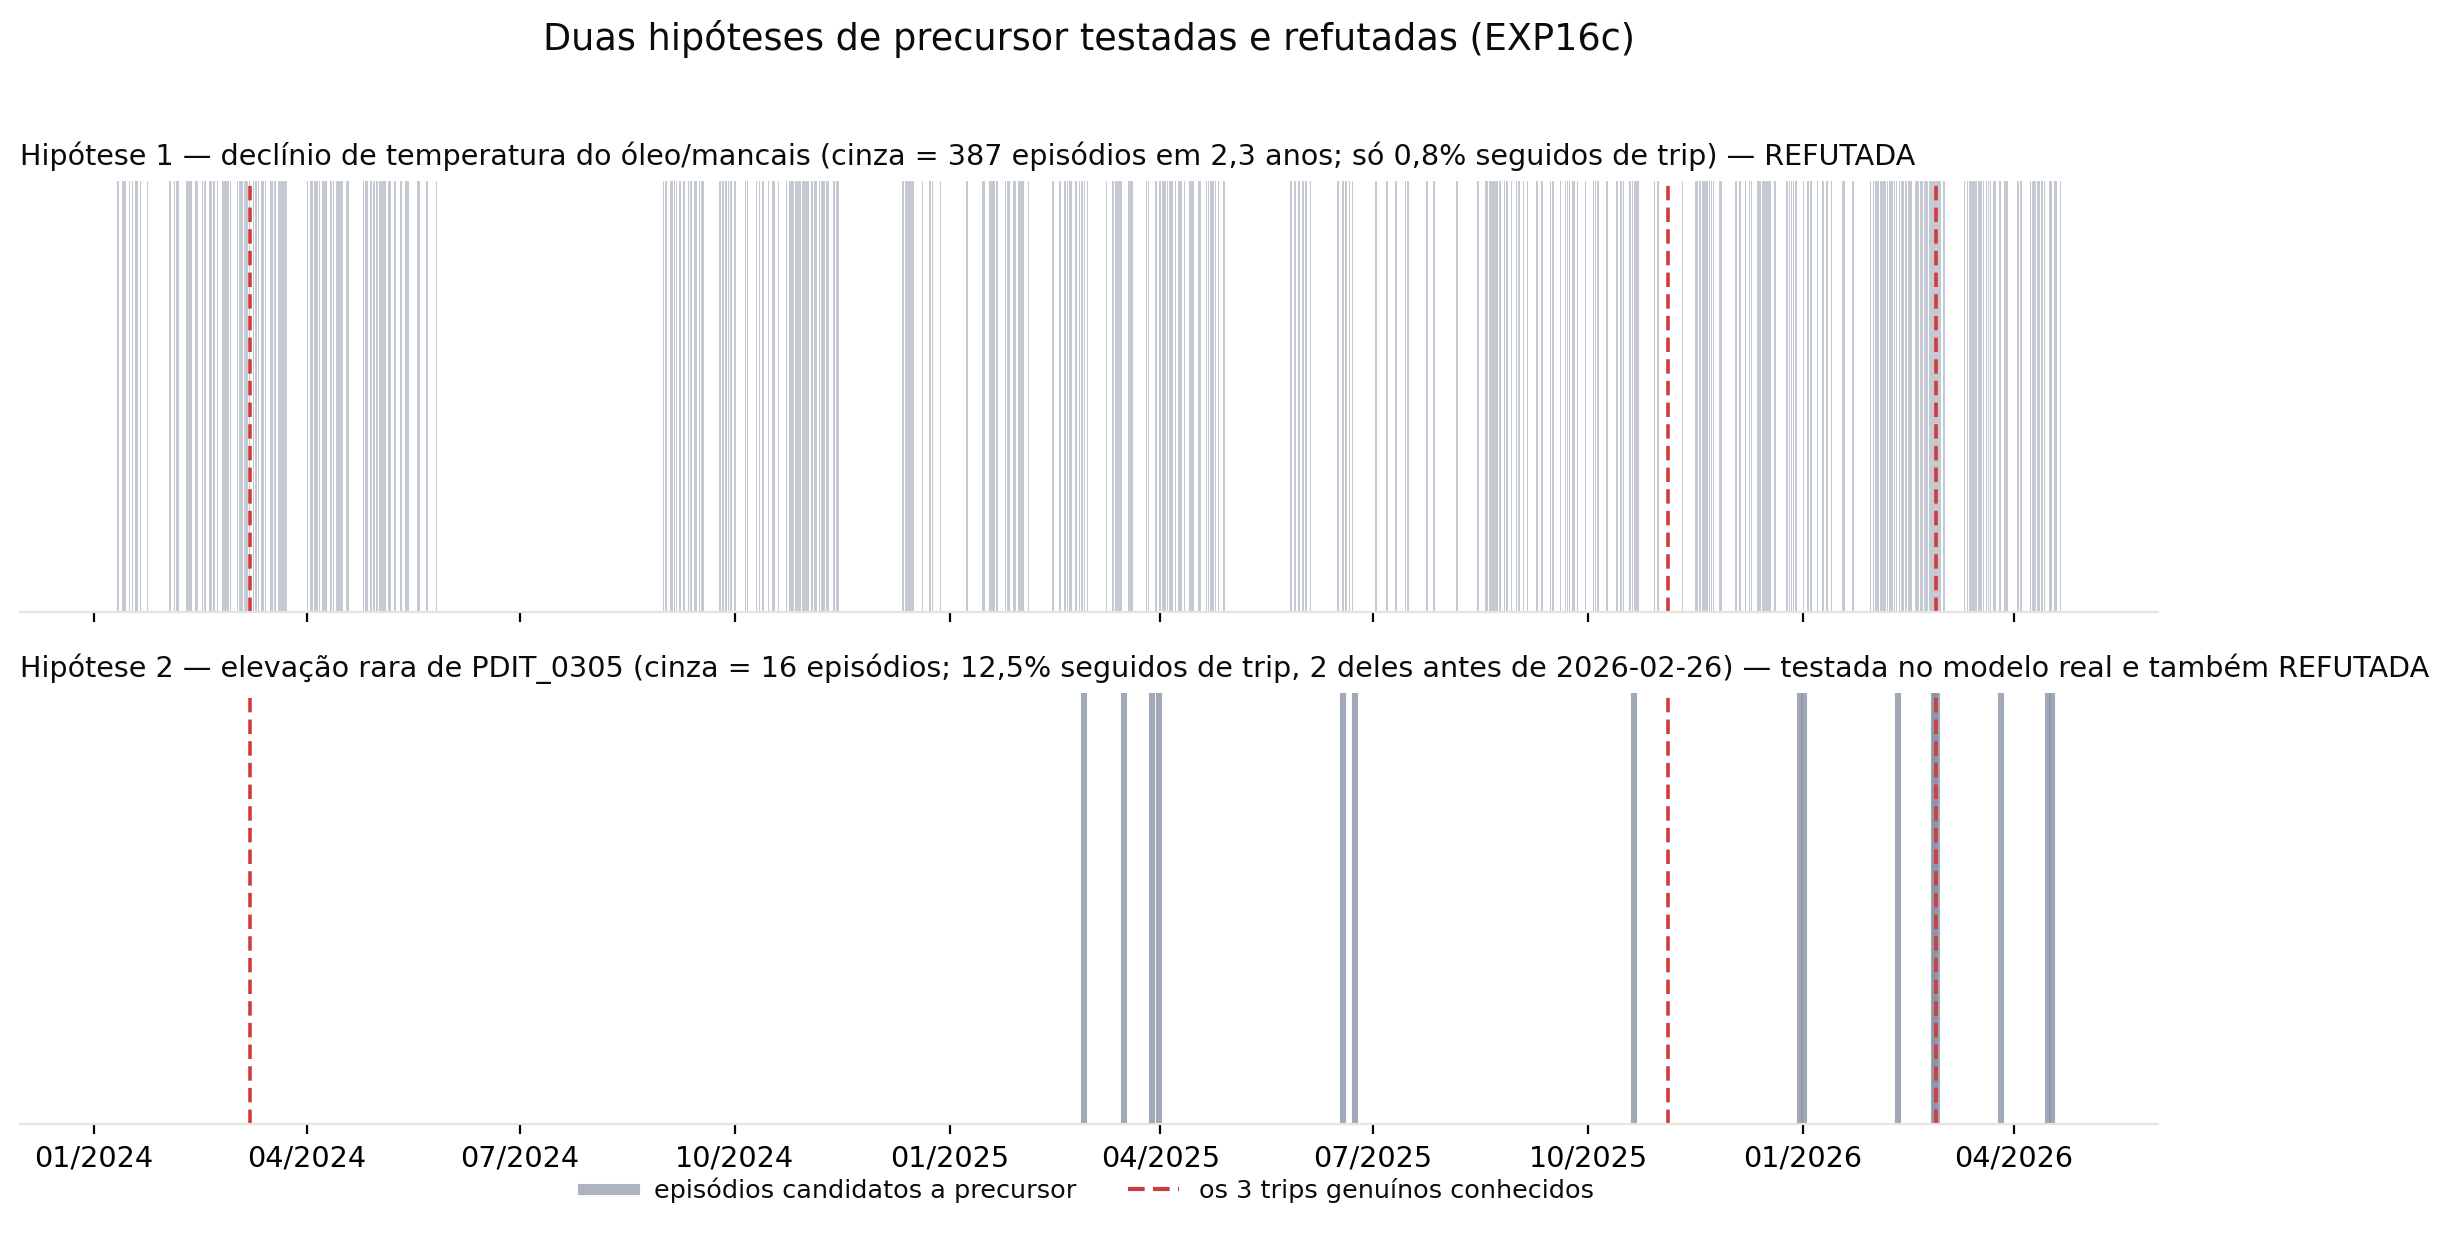
\includegraphics[width=\textwidth]{fig_precursores_refutados.png}
\caption{As duas hipóteses testadas, mostradas na linha do tempo completa.
A Hipótese 1 (declínio de temperatura) ocorre com tanta frequência que é
essencialmente ruído operacional. A Hipótese 2 (\texttt{PDIT\_0305}) é
rara e por isso mais promissora à primeira vista, mas ao ser incorporada
de fato ao modelo (não apenas observada isoladamente), não mudou o
resultado.}
\label{fig:precursores}
\end{figure}

\paragraph{Hipótese 1 -- declínio de temperatura do óleo/mancais.}
Nas $\sim$20h antes do evento de 2024-03-07, as 5 temperaturas do sistema
de lubrificação (\texttt{TI\_0301}, \texttt{TI\_0303}, \texttt{TI\_0305},
\texttt{TI\_0307}, \texttt{TI\_0325}) caem de forma coerente entre si
($\sim$1,5--2°C). À primeira vista, parece um resfriamento real do
sistema. Uma checagem de \textbf{taxa-base} sobre todo o histórico, porém,
mostrou que esse padrão de queda simultânea ocorre em \textbf{387
episódios distintos, 32,5\% de todo o tempo operacional} -- e só 0,8\%
desses episódios são seguidos de um trip. É variação normal (provavelmente
ligada a ciclo diário/carga), não um precursor. Confirmou-se ainda que o
modelo multivariado já treinado (que já incluía essas 5 temperaturas como
feature) não sinalizou absolutamente nada nessa janela específica --
\textbf{refutada}.

\paragraph{Hipótese 2 -- elevação de \texttt{PDIT\_0305} (pressão diferencial
de vazamento de gás de selagem).}
Um segundo candidato pareceu bem mais específico: o valor de
\texttt{PDIT\_0305} cruza $0{,}3$ em apenas \textbf{16 episódios em 2,3
anos (0,036\% do tempo)}, dos quais \textbf{2 precedem diretamente} o
evento de 2026-02-26 (um $\sim$20h antes, outro $\sim$4,5h antes) -- uma
taxa de conversão de 12,5\%, ordens de grandeza mais específica que a
Hipótese 1. Motivado por esse achado, o EXP16c treinou o modelo real
adicionando \texttt{PDIT\_0305} ao grupo de sensores e comparou o
resultado ponto a ponto contra o modelo sem essa feature:

\begin{center}
\begin{tabular}{lcc}
\toprule
& Sem \texttt{PDIT\_0305} & Com \texttt{PDIT\_0305} \\
\midrule
Primeiro ponto anômalo em 2026-02-26 & 22h17 (6,7h \emph{depois}) & 22h17 (6,7h \emph{depois}) \\
Pontos anômalos na janela & 26 & 32 \\
\bottomrule
\end{tabular}
\end{center}

O resultado não mudou -- a antecedência continua idêntica (nenhuma, o
ponto ainda aparece só depois do trip). O sinal correto na análise de
taxa-base não sobreviveu ao score conjunto do \texttt{IsolationForest} com
os outros 11 sensores, provavelmente diluído pela mesma dinâmica que
descartou a Hipótese 1. \textbf{Também refutada}, mas de forma mais
rigorosa: não só por taxa-base, mas confirmada diretamente no modelo real.

\paragraph{Conclusão desta investigação.} Duas hipóteses concretas,
levantadas a partir de uma varredura sistemática de $\sim$36 sensores e
testadas com o rigor de (a) checagem de taxa-base contra todo o histórico e
(b) confirmação no modelo real treinado, foram refutadas. Isso fecha, por
ora, o ciclo de busca por precursores baratos para os 2 casos sem sinal --
mesma categoria de achado negativo já documentada para a série de
experimentos da T5 (EXP13). Não há evidência de que mais tempo de busca
nos sensores já disponíveis destrave esses 2 casos.

\section{Discussão}

\subsection{Este modelo prediz \emph{todas} as falhas desse tipo?}

Não. Mesmo supondo uma engenharia de deploy perfeita (dado em tempo real,
retreino contínuo, alerta operacional funcionando), este modelo, com este
conjunto de sensores, teria previsto historicamente \textbf{1 dos 3 trips
genuínos conhecidos ($\sim$33\%)}. Não é uma limitação de engenharia -- é
um limite de informação: nos outros 2 casos, a pressão fica completamente
estável até o instante em que o problema já aconteceu. É plausível que
esse tipo de trip tenha duas causas físicas distintas -- uma degradação
lenta e detectável, e um evento abrupto/mecânico sem aviso --, e o modelo
só consegue captar a primeira com a instrumentação atual.

\subsection{Prontidão para produção}

O pipeline atual é retrospectivo/batch, não um serviço de inferência
contínua. Faltam, no mínimo: conexão viva com o historian de processo,
job de scoring agendado, integração com alerta operacional, e uma rotina
de retreino periódico (o modelo aprendeu ``normal'' só até jun/2025, sem
atualização desde então). Some-se a isso a base de validação pequena
(n=2--3), e o resultado deste relatório deve ser lido como uma
\textbf{prova de conceito que confirma sinal real} (o caso de 14h de
antecedência), não como um sistema pronto para proteger a operação.

\subsection{Limitações e pendências}

\begin{itemize}[leftmargin=1.4em]
  \item Amostra de avaliação muito pequena (n=2 no teste, n=3 no total
  conhecido) -- qualquer taxa de acerto carrega incerteza estatística
  grande.
  \item Não foi encontrada fonte de dado para ampliar a janela histórica
  (2023 está ausente nos datasets ClearML disponíveis).
  \item 16 episódios de falso alerta residual (0,143\%) foram
  caracterizados: mistura de manobras de carga reais, 1 glitch de sensor
  confirmado, e o restante sem causa identificada com os sinais checados.
  \item Um config de referência em CNN1D-Autoencoder foi preparado mas não
  chegou a ser necessário, dado o desempenho já forte do AutoML/\texttt{iforest}.
\end{itemize}

\section{Conclusão}

O EXP16 estabeleceu, pela primeira vez, uma pipeline de detecção para o
alarme de trip de óleo lubrificante do compressor, independente da linha
de trabalho da T5. O modelo vencedor -- \texttt{IsolationForest} sobre o
alvo mais os 10 canais de vibração, sem nenhum portão de pós-processamento
-- atinge falso alerta baixo (0,143\%) e variância de semente nula, e
demonstrou capacidade preditiva real em pelo menos um episódio histórico
(14,3 horas de antecedência). A investigação foi além da métrica agregada:
verificou a antecedência real ponto a ponto, testou e refutou duas
hipóteses concretas de precursor para os casos sem detecção, e chegou a
uma conclusão honesta sobre os limites do que a instrumentação atual
permite prever -- $\sim$1 em 3 casos, não a totalidade dos trips deste
tipo.

\section{Tasks ClearML referenciadas}

\begin{itemize}[leftmargin=1.4em]
  \item \texttt{15833383325746c999e8b866dda4b5e9} -- EXP16a, grid amplo de
  AutoML (840 trials), vencedor \texttt{iforest} identificado.
  \item \texttt{fc787faca377406890fed0309cd95b3c} -- EXP16b, config final
  travado + seed-sweep (5 sementes, variância zero).
  \item \texttt{640251258fcc471bb8f25bf8fe3ffac8} e
  \texttt{3f679264f5cb4c2081f658bdb2fa154b} -- EXP16c, teste da hipótese
  \texttt{PDIT\_0305} (refutada).
\end{itemize}

\end{document}
